
\twocolumn[{%
\begin{center}
  {\LARGE \textbf{\textsf{Top Quark Seminar I}}} \\
  \vspace{1em}
  {\Large \textbf{\textsf{Igor Babuschkin}}} \\
  \vspace{1em}
  {\large \textbf{\textsf{4th January 2015}}}
  \section*{Summary of \enquote{Search for the Top Quark: Results from the DØ Experiment}}
\end{center}
}]

The paper\cite{dzero} constitutes part of the proceedings of a 1994 high energy physics conference in Glasgow.
It documents the progress that the DØ collaboration had made in the search for the top quark, which at that point had not been discovered, but was strongly suspected to exist.
More precisely, the paper describes an analysis using data taken over the years 1992 and 1993 with $\SI{13.5}{\pico\barn}^{-1}$ of integrated luminosity at the Tevatron (a $\Pp\Pap$ collider).
The analysis looked for $\Pqt\APqt$ pairs via dilepton plus jets and single leptons plus jets final states.
The preliminary results presented at the conference did not suffice to claim a discovery of the top quark with the necessary statistical significance.

It is interesting to note that, in contrast to the LHC, the dominant \Pqt\!\!\APqt production mechanism at the Tevatron was $q\overline{q}$ annihilation, while gluon fusion had a smaller role.
This was caused by the fact that protons were collided with antiprotons, in addition to the lower center-of-mass energy.

The paper cites \SI{131}{GeV/c^2} as the best previous lower limit for the top quark mass $m_{\Pqt}$.
It also refers to results by the CDF collaboration\cite{cdf} suggesting that the top quark mass would lie in the range \SIrange{160}{190}{GeV/c^2}.

The analysis is based on three strategies: Searching for dilepton events, for single lepton events via topological properties of the event, and for single lepton events using \Pqb-tagging, which was a novel technique at the time.

\Pqb-tagging is a technique for identifying jets that contain \Pqb-quarks.
For example, a jet can be tagged by identifying a muon that originates from it (and not from the primary interaction).

To separate background events from signal candidates, various cuts are applied to the dataset.
These select leptons with high transverse momentum, events with large missing transverse energy, and various other properties.

After applying the cuts, only 7 signal candidates remain in total (from all three strategies), while 3 background events are expected.
This excess was not enough to claim a discovery of the top quark.
While the corresponding CDF analysis had a sensitivity comporable to that of DØ, they measured a larger number of signal candidates\cite{cdf}.
The results from DØ and CDF are displayed in figure \ref{results}.

Finally, the author points out that the presented results were preliminary, that the analysis would be improved in the future (for example by using multivariate analysis techniques), and that further data would be taken at the Tevatron.

\begin{figure}
  \centering
  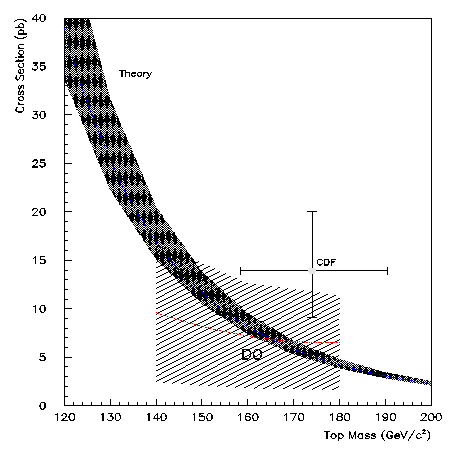
\includegraphics[width=0.4\textwidth]{figures/result.pdf}
  \caption{
    Preliminary results for the $\Pqt\APqt$ cross section from DØ and CDF, compared to the theoretical prediction depending on the top quark mass.
  }
  \label{results}
\end{figure}
